% LLNCS macro package for Springer Computer Science proceedings;
% Version 2.20 of 2017/10/04
%
\documentclass[runningheads]{llncs}
%
\usepackage{graphicx}
% Used for displaying a sample figure. If possible, figure files should
% be included in EPS format.
%
% If you use the hyperref package, please uncomment the following line
% to display URLs in blue roman font according to Springer's eBook style:
% \renewcommand\UrlFont{\color{blue}\rmfamily}

% My packages
\usepackage{orcidlink} % Orcid links
\newcommand\Mark[1]{\textsuperscript#1}

\usepackage{amssymb} % \square command
% Footnotes inside tables
\usepackage{footnote}
\usepackage{csquotes} % enquote command
\usepackage{glossaries} % Glossary
\usepackage{threeparttable} % Tables with notes
\makesavenoteenv{tabular}
\makesavenoteenv{table}
% Acronyms
\newacronym{bpmn}{BPMN}{Business Process Modeling Notation}
\newacronym{gt}{GT}{Graph Transformation}
\newacronym{mt}{MT}{Model Transformation}
\newacronym{hot}{HOT}{Higher-Order model Transformation}
% Fix underscore in dois
\usepackage[strings]{underscore}

\begin{document}
%
\title{Formalization and analysis of BPMN using graph transformation systems}
%
%\titlerunning{Abbreviated paper title}
% If the paper title is too long for the running head, you can set
% an abbreviated paper title here
%
\author{Tim Kr\"{a}uter\inst{1}\orcidlink{0000-0003-1795-0611} \and
Adrian Rutle\inst{1}\orcidlink{0000-0002-4158-1644} \and
Harald K\"{o}nig\inst{2,1}\orcidlink{0000-0001-6304-6311} \and
Yngve Lamo\inst{1}\orcidlink{0000-0001-9196-1779}}
%
\authorrunning{T. Kräuter et al.}
% First names are abbreviated in the running head.
% If there are more than two authors, 'et al.' is used.
%
\institute{Western Norway University of Applied Sciences, Bergen, Norway 
\email{tkra@hvl.no, aru@hvl.no, yla@hvl.no} \and
University of Applied Sciences, FHDW, Hanover, Germany\\
\email{harald.koenig@fhdw.de}}
%
\maketitle              % typeset the header of the contribution
%
\begin{abstract}
The Business Process Modeling Notation (BPMN) is a widely used standard notation for defining intra- and inter-organizational workflows.
However, the informal description of the BPMN execution semantics leads to different interpretations of BPMN features and difficulties in checking behavioral properties.
In this paper, we propose a formalization of the execution semantics of BPMN that, compared to existing approaches, covers more BPMN features while allowing property checking.
Our approach is based on a higher-order transformation from BPMN models to graph transformation systems.
As proof of concept, we have implemented our approach in an open-source web-based tool.

\keywords{BPMN \and Model transformation \and Graph transformation \and Model checking \and Formalization}
\end{abstract}

% TODO: Add discussion section with benchmark.

\section{Introduction}
\gls*{bpmn} \cite{objectmanagementgroupBusinessProcessModel2013} is a widely used standard notation to define intra- and inter-organizational workflows.
However, the informal description of the BPMN execution semantics leads to different interpretations of BPMN features and difficulties in checking behavioral properties \cite{corradiniFormalApproachAnalysis2021}.
One can detect errors and optimization potential in process models already during their creation by checking behavioral properties.
Thus, the cost of business process automation using \gls*{bpmn} can be reduced.
Consequently, we propose a formalization that covers most of the \gls*{bpmn} features used in practice and supports checking behavioral properties.

Generally, we think about two fundamental concepts when formalizing the execution semantics of a behavioral language.
First, \textit{state structure}, i.e., how can one represent models during execution.
The state structure corresponds to the typegraph in \gls*{gt} systems.
Second, \textit{state-changing elements}, i.e., which elements in a model encode potential state changes.
Those elements must then be implemented using \gls*{gt} rules.
Our approach creates \gls*{gt} rules based on a \gls*{hot} and is summarized in \autoref{fig:approach}.

% Describe the approach and highlight that it can be generalized to other languages with state and state-changing elements.
\begin{figure}[ht]
    \centering
    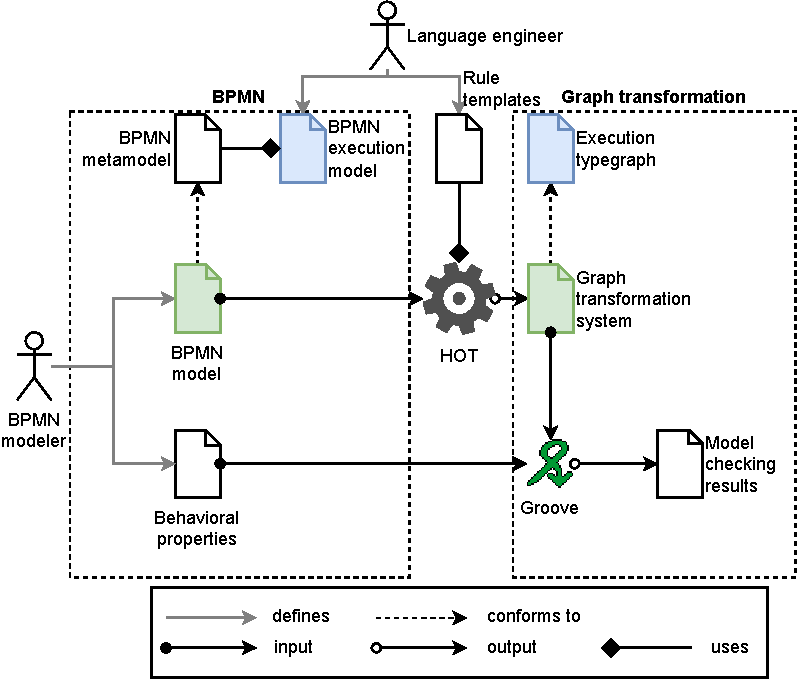
\includegraphics[width=0.8\textwidth]{images/bpmn_semantics-overview.pdf}
    \caption{Overview of the approach}
    \label{fig:approach}
\end{figure}

First, a modeler defines a BPMN model and behavioral properties to check.
The BPMN model conforms to the BPMN metamodel defined in the BPMN specification \cite{objectmanagementgroupBusinessProcessModel2013}.
Using the BPMN metamodel, we define the state structure for BPMN in a so-called BPMN execution metamodel, fulfilling the role of a language engineer.
Usually, an execution metamodel is defined by extending the structural metamodel.

Furthermore, we define a \gls*{hot} from BPMN models to \gls*{gt} systems.
We call the transformation \textit{higher-order} since the resulting graph-transformation systems represent model-transformations themselves \cite{tisiUseHigherOrderModel2009}.
The \gls*{hot} creates a \gls*{gt} system, i.e., \gls*{gt} rules and a start graph for a given BPMN model.
It is defined using so-called rule generation templates, which describe how \gls*{gt} rules should be generated for each state-changing element in BPMN (see \autoref{sec:formalization}).
The obtained \gls*{gt} system conforms to the execution type graph representing the BPMN execution model interpreted as a type graph.
We colored both artifacts in blue to visualize that they contain the same information.
Finally, we check the previously defined behavioral properties using Groove to run the \gls*{gt} system.

We implemented our approach in an open-source web-based tool such that it is easily accessible without needing any local installation.
Furthermore, our approach is general since it can be used to formalize other behavioral languages.
To formalize the execution semantics of a different behavioral language, one only needs to define a new execution metamodel and \gls*{hot} (see language engineer in \autoref{fig:approach})

% Paper outline
The remainder of this paper is structured as follows.
First, in \autoref{sec:preliminaries}, we introduce \gls*{bpmn} and point out the theoretical background of this contribution.
Second, we describe the \gls*{bpmn} semantics formalization using the \gls*{hot} (\autoref{sec:formalization}) before explaining how this can be utilized for model checking BPMN-specific and custom properties (\autoref{sec:modelChecking}).
Then, in \autoref{sec:impl}, we present the web-based tool implementing our approach.
Finally, we discuss related work regarding BPMN feature coverage in \autoref{sec:relatedWork} and conclude in \autoref{sec:conclusion}.

\section{Preliminaries} \label{sec:preliminaries}
In this paper, we apply \gls*{gt}s to formalize the execution semantics of BPMN.
Thus, in this section, we will briefly introduce BPMN and its execution semantics.
Please refer to \cite{freundRealLifeBPMNUsing2019} or the BPMN specification \cite{objectmanagementgroupBusinessProcessModel2013} for further information about BPMN.
Furthermore, we outline the theoretical background behind our application of \gls*{gt}s.
\subsection{BPMN}
\autoref{fig:bpmnMetamodel} depicts the structure of BPMN models with the corresponding concrete syntax BPMN symbols contained in clouds.

\begin{figure}[ht]
  \centering
  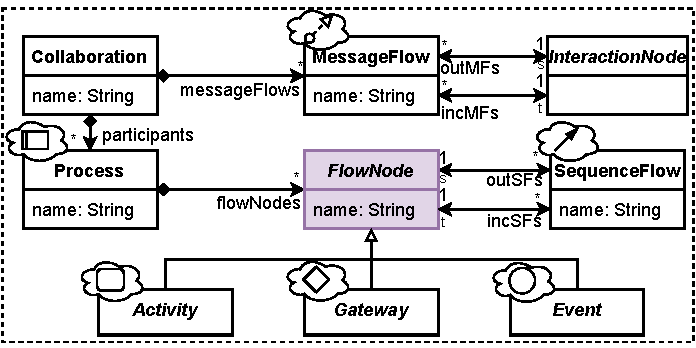
\includegraphics[width=0.75\linewidth]{images/bpmn_semantics-bpmn-metamodel.pdf}
  \caption{Excerpt of the BPMN metamodel \cite{objectmanagementgroupBusinessProcessModel2013}}
  \label{fig:bpmnMetamodel}
\end{figure}

A BPMN model is represented by a \textsf{Collaboration} that has \textsf{participants} and \textsf{MessageFlows} between \textsf{InteractionNodes} (see  \autoref{fig:bpmnMetamodel}).
Each participant is a \textsf{Process} containing \textsf{FlowNodes} connected by \textsf{SequenceFlows}.
A \textsf{FlowNode} is either an \textsf{Activity}, \textsf{Gateway}, or \textsf{Event}.
Many types of \textsf{Activities}, \textsf{Gateways}, and \textsf{Events} exist.
Activities represent certain tasks to be carried out during a process, while events may happen during the execution of these tasks.
Furthermore, gateways model conditions, parallelizations, and synchronizations \cite{freundRealLifeBPMNUsing2019}.

% BPMN semantics: Token distribution
The BPMN execution semantics are described using the concept of \emph{tokens} \cite{objectmanagementgroupBusinessProcessModel2013}, which can be located at sequence flows and specific flow nodes.
Tokens are consumed and created by flow nodes according to the connected sequence flows.
Thus, the flow nodes are colored purple in \autoref{fig:bpmnMetamodel} since they are the \textit{state-changing elements} of BPMN and are crucial when formalizing the BPMN execution semantics in \autoref{sec:formalization}.
A BPMN process is triggered by one of its start events, leading to the creation of a token at the triggered start event.
% Activities
Activities can start when at least one token is located on an incoming sequence flow.
The start of an activity will move the incoming token to the activity.
When an activity finishes, it deletes its token and adds one at each outgoing sequence flow.
% Gateways
Furthermore, different gateway types exist, such as parallelization, synchronization, XOR, and OR distribution of tokens.
% Events (basic)
Events delete and add tokens similar to activities but have additional semantics depending on their type.
For example, message events will add or delete messages.

\subsection{Theoretical background}
We use typed attributed graphs for the formalization of the BPMN execution semantics.
Each state, i.e., token distribution during the execution of a BPMN model, is represented as an attributed graph typed by the BPMN execution type graph, which is introduced in \autoref{sec:formalization}.

% Groove uses the single pushout approach with negative application conditions.
Regarding \gls*{gt}, we utilize the single-pushout (SPO) approach with negative application conditions (NAC) \cite{ehrigALGEBRAICAPPROACHESGRAPH1997}.
In addition, we utilize \emph{nested rules} with quantification to make parts of a rule applied repeatedly or optionally \cite{rensinkNestedQuantificationGraph2006,rensinkHowMuchAre2017}.
Moreover, we utilize NACs to implement more intricate parts in the BPMN execution semantics, such as the termination of processes. 
In SPO rewriting, a \gls*{gt} rule is defined as a partial graph morphism $L \to R$, where in our case, $L$ and $R$ are typed attributed graphs. 



\section{BPMN semantics formalization} \label{sec:formalization}

Since our approach is based on a \gls*{hot} from BPMN to \gls*{gt} systems, we generate a \emph{start graph} and \emph{\gls*{gt} rules} for a given BPMN model.
The approach supports the BPMN features depicted in \autoref{fig:bpmnfeaturesOverview}.
BPMN features are divided into \textsf{Events}, \textsf{Gateways}, \textsf{Activities}, and \textsf{Edges}.
\textsf{Events} and \textsf{Activities} are further divided into subgroups.
Due to space limitations, we only explain how the features marked with a green background are realized in this paper.
However, the other features are also implemented and tested \cite{krauterArtifactsICGT2023}.

\begin{figure}[ht]
    \centering
    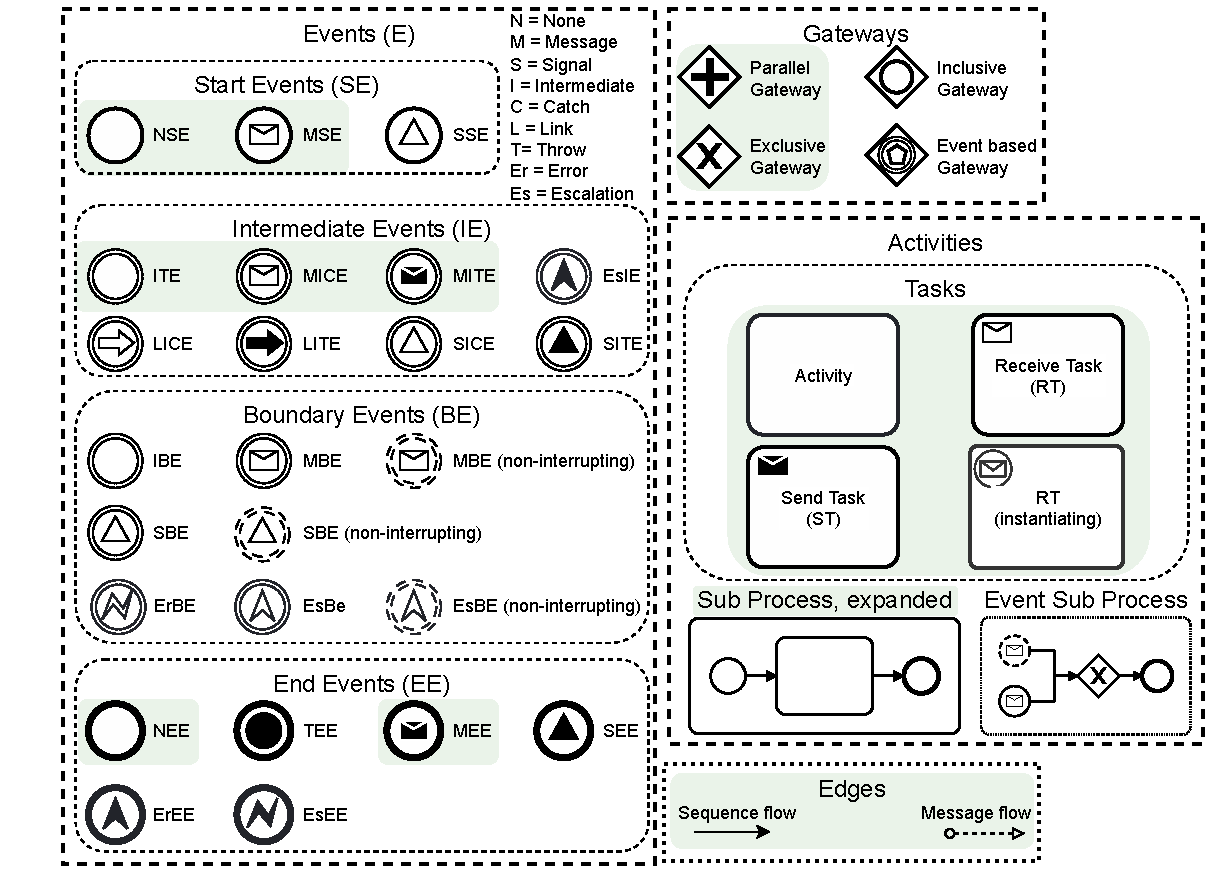
\includegraphics[width=0.99\textwidth]{images/bpmn_semantics-feature-overview.pdf}
    \caption{Overview of the supported BPMN features (structure adapted from \cite{houhouFirstOrderLogicVerification2022})}
    \label{fig:bpmnfeaturesOverview}
\end{figure}

Before we explain our implementation of the BPMN features, we define the BPMN execution metamodel.

\subsection{BPMN execution metamodel}

Our formalization of BPMN is token-based, as in the informal description of the BPMN specification \cite{objectmanagementgroupBusinessProcessModel2013}.
Thus, to describe processes holding tokens during execution, we use the type graph shown in \autoref{fig:typeGraph}.
The type graph is depicted as a UML class diagram without operations, which can be seen as an attributed type graph with inheritance \cite{heckelGraphTransformationSoftware2020}.

\begin{figure}[ht]
  \centering
  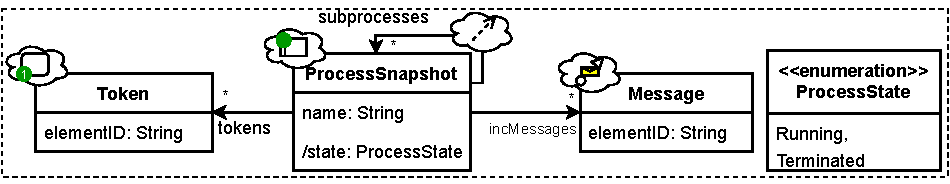
\includegraphics[width=0.5\linewidth]{images/bpmn_semantics-typegraph.pdf}
  \caption{BPMN execution metamodel}
  \label{fig:typeGraph}
\end{figure}

We use \textsf{ProcessSnapshot} to denote a running BPMN process with a specific token distribution that describes one state in the history of process states during the execution.
Every \textsf{ProcessSnapshot} has a set of \textsf{tokens}, incoming \textsf{messages}, and \textsf{subprocesses}.
A \textsf{ProcessSnapshot} has the state \textsf{Terminated} if it has no \textsf{tokens} or \textsf{subprocesses}.
Otherwise, it has the state \textsf{Running}.
A \textsf{Token} has an \textsf{elementID}, which points to the BPMN \textsf{Activity} or the \textsf{SequenceFlow} at which it is located.
A \textsf{Message} has an \textsf{elementID} pointing to a \textsf{MessageFlow}.
To concisely depict graphs conforming to this type graph, we introduce a concrete syntax in the clouds attached to the elements.
Our concrete syntax extends the BPMN syntax by adding process snapshots, subprocess relations, tokens, and messages.
Tokens are represented as colored circles drawn at their specified positions in a model.
In addition, we use colored circles at the top left of the bounding box, representing instances of the BPMN \textsf{Process}; these circles represent process snapshots.
% Token color must match the tokens relation in the type graph (constraint!). This should be checked by the tool when using concrete syntax.
The token's color must match the color of the process snapshot holding the token.
The concrete syntax was inspired by the bpmn-js-token-simulation\footnote{\url{https://github.com/bpmn-io/bpmn-js-token-simulation}}.
Using this type graph, we can now define how the start graph and graph-transformation rules for the different BPMN features are created.

% How is a start graph generated?
The generation of the start graph for a BPMN model is straightforward.
First, for each process in the BPMN model, we generate a process snapshot if the process contains a none start event (NSE).
A NSE describes a start event without a trigger (none).
Popular start event triggers are message and signal (see MSE and SSE in \autoref{fig:bpmnfeaturesOverview}).
Then, for each NSE, we add a token to the respective process snapshot.
An example of a start graph is shown in \autoref{fig:startGraph} using abstract and concrete syntax.
Furthermore, we consider allowing the user to define a start graph similar to how he can define atomic propositions for custom properties (see \autoref{subsec:customProperties}).

\begin{figure}[ht]
    \centering
    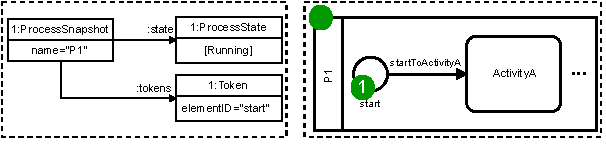
\includegraphics[width=0.7\textwidth]{images/startGraph.pdf}
    \caption{Example start graph in abstract (left) and concrete syntax (right)}
    \label{fig:startGraph}
\end{figure}

The \gls*{hot} generates one or more \gls*{gt} rules for each \textsf{FlowNode} in a BPMN model.
To give an intuition about the transformation, we will first describe example results, i.e., generated rules for an NSE, a task, a \textit{message intermediate catch event} (MICE), and a \textit{message intermediate throw event} (MITE) (see \autoref{fig:bpmnfeaturesOverview}).
Afterward, we will explain how these---and other---rules are created by our \gls*{hot}.

\autoref{fig:gtRuleAbstract} depicts an example \gls*{gt} rule ($L \to R$) for an NSE in abstract syntax.
The rule is straightforward and moves a token from the start event to its outgoing sequence flow.
For the rest of the paper, we will depict all rules in the concrete syntax introduced earlier.
The rule from \autoref{fig:gtRuleAbstract} depicted in concrete syntax is shown in \autoref{fig:gtRuleConcrete}.

\begin{figure}[ht]
    \centering
  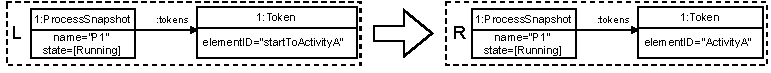
\includegraphics[width=0.8\textwidth]{images/rule_abstract.pdf}
  \caption{Example \gls*{gt} rule for an NSE (abstract syntax)}  \label{fig:gtRuleAbstract}
\end{figure}

\begin{figure}[ht]
    \centering
  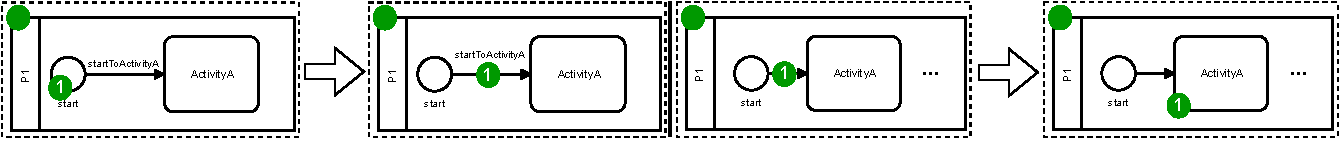
\includegraphics[width=0.6\textwidth]{images/rule_concrete.pdf}
  \caption{Example \gls*{gt} rule for an NSE (concrete syntax)}
  \label{fig:gtRuleConcrete}
\end{figure}

The rule in \autoref{fig:taskRules} represents the start of a task, which will move one token from the incoming sequence flow to the task itself.

\begin{figure}[ht]
    \centering
    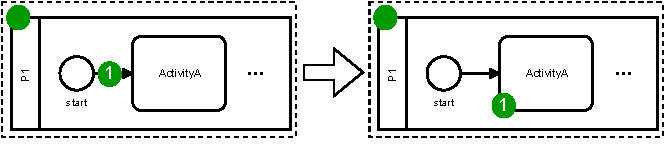
\includegraphics[width=0.6\textwidth]{images/bpmn_semantics-rules.pdf}
    \caption{Example \gls*{gt} rule to start a task.}
    \label{fig:taskRules}
\end{figure}

The left rule in \autoref{fig:messageEventRules} realizes a MITE, and the right rule implements a MICE.
The MITE rule moves the token through the event and may send a message to a waiting process snapshot if it has a token waiting at the corresponding MICE.
An optional existential quantifier \cite{rensinkNestedQuantificationGraph2006} is used to send a message only if the receiving process is ready to receive it.
The MICE rule deletes a token and a message and adds an outgoing token.

\begin{figure}[ht]
    \centering
    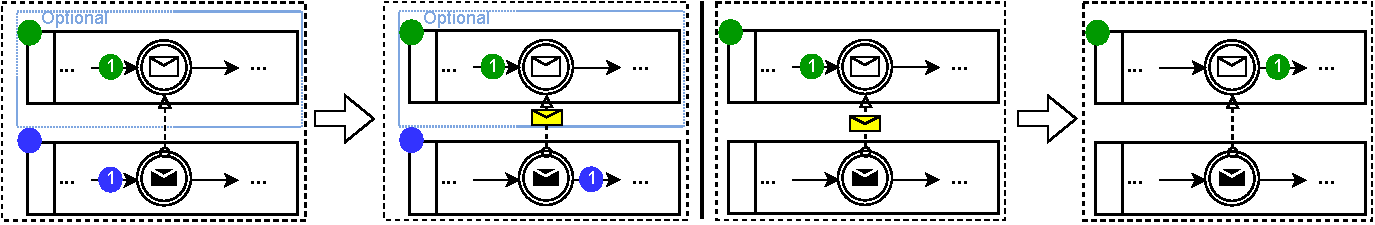
\includegraphics[width=1\textwidth]{images/bpmn_semantics-message-events.pdf}
    \caption{Rules for MITE (left) and MICE (right)}
    \label{fig:messageEventRules}
\end{figure}

To summarize, we described four example rules and introduced a concrete syntax to depict them concisely and understandably.
In the following subsections, we use this concrete syntax to describe how these rules and rules for other flow nodes are generated by our \gls*{hot}.
Elements of the \gls*{hot} are depicted using rule generation templates that describe how specific rules are created for various flow nodes.
We only explain rule generation for (i) process instantiation and termination, (ii) activities and subprocesses, (iii) gateways, as well as (iv) message events due to space constraints.
However, our implementation covers all concepts shown in \autoref{fig:bpmnfeaturesOverview}.


\subsection{Process instantiation and termination} \label{subsec:instAndTermination}

\autoref{fig:startAndEndTemplate} depicts the rule generation templates for start and end events (\textsf{NSE} and \textsf{NEE} in \autoref{fig:bpmnfeaturesOverview}).
All rule generation templates show a BPMN structure defined in the left column and the applicable rule generation template in the right column.
The structures in the left column show instances of the BPMN metamodel (\autoref{fig:bpmnMetamodel}), and the ones in the right column show the generated rules typed by the BPMN execution type graph (see \autoref{fig:typeGraph}).
If more than one rule is generated from a BPMN structure there is an expression defining how each rule is generated.
For example, the expression $\forall \text{sf} \in \text{E.incSFs}$ for the rule generation template of end events (see \autoref{fig:startAndEndTemplate}) generates one rule for each incoming sequence flow \textit{sf} of the end event \textit{E}.
We use "." in expressions to navigate along the associations of the BPMN metamodel \autoref{fig:bpmnMetamodel}.
In the example, \textsf{E.incSFs} means following all \textsf{incSFs} links for a \textsf{FlowNode} object, resulting in a set of \textsf{SequenceFlow} objects.



\begin{figure}[ht]
    \centering
    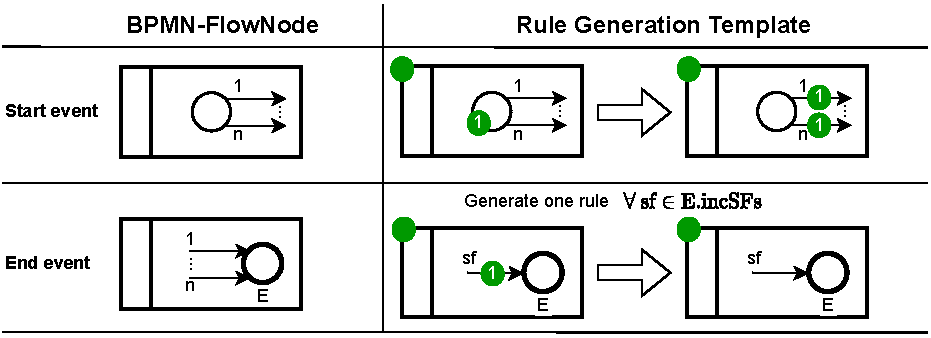
\includegraphics[width=.9\textwidth]{images/start_end_template.pdf}
    \caption{Rule generation templates for start and end events}
    \label{fig:startAndEndTemplate}
\end{figure}

% Start Event + Refer to the start graph.
The start event rule template generates the start event rule in \autoref{fig:gtRuleConcrete}.
The tokens located on the start events are deleted by start event rules, while one token for each outgoing sequence flow is added.
If a start event has more than one outgoing sequence flow, it functions as an \textit{implicit parallel gateway}, forking the control flow by creating one token for each of the sequence flows.
Initially, the tokens on the start events are given by the start graph of the \gls*{gt} system (see, e.g., \autoref{fig:startGraph}).
    
% End Event
The generated end event rules delete tokens one by one for each incoming sequence flow.
However, they do not terminate processes.
% General termination rule
Process termination is implemented with a generic rule---independent of the input BPMN model---which is applicable to all process snapshots.
The termination rule (see \autoref{fig:terminationRule}) is automatically generated once during the \gls*{hot}.
It is used to terminate processes and subprocesses if they do not have any tokens.
The rule uses a NAC only to change the state of the process snapshot from running to terminated if it has no tokens and subprocesses.
The concrete termination rule in Groove is given as an artifact \cite{krauterArtifactsICGT2023}.

\begin{figure}[ht]
    \centering
    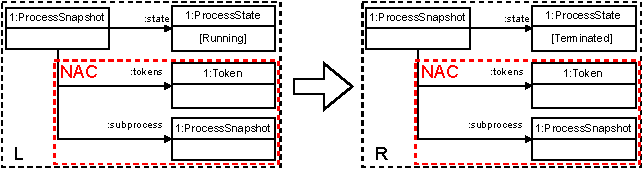
\includegraphics[width=.8\textwidth]{images/bpmn_semantics-termination_rule.pdf}
    \caption{Termination rule}
    \label{fig:terminationRule}
\end{figure}

\subsection{Activities \& Subprocesses}

% Normal activities
\autoref{fig:activityTemplates} depicts the rule generation templates for activities and subprocesses (see \autoref{fig:bpmnfeaturesOverview}).
Activity execution is divided into two steps implemented by two rule templates.
The upper template generates one rule for each incoming sequence flow to start the activity.
An activity can be started using a token positioned at any of its incoming sequence flows.
Thus, multiple incoming sequence flows represent an \textit{implicit exclusive gateway} (see exclusive gateway in \autoref{fig:gatewayTemplates}).
This rule template generates the sample rule in \autoref{fig:taskRules}.

The bottom rule template generates one rule that ends the activity.
It deletes a token at the activity and adds one token at each outgoing sequence flow.
Like start events, this implicitly encodes the same forking behavior as a parallel gateway (see \autoref{fig:gatewayTemplates}). 

\begin{figure}[ht]
    \centering
    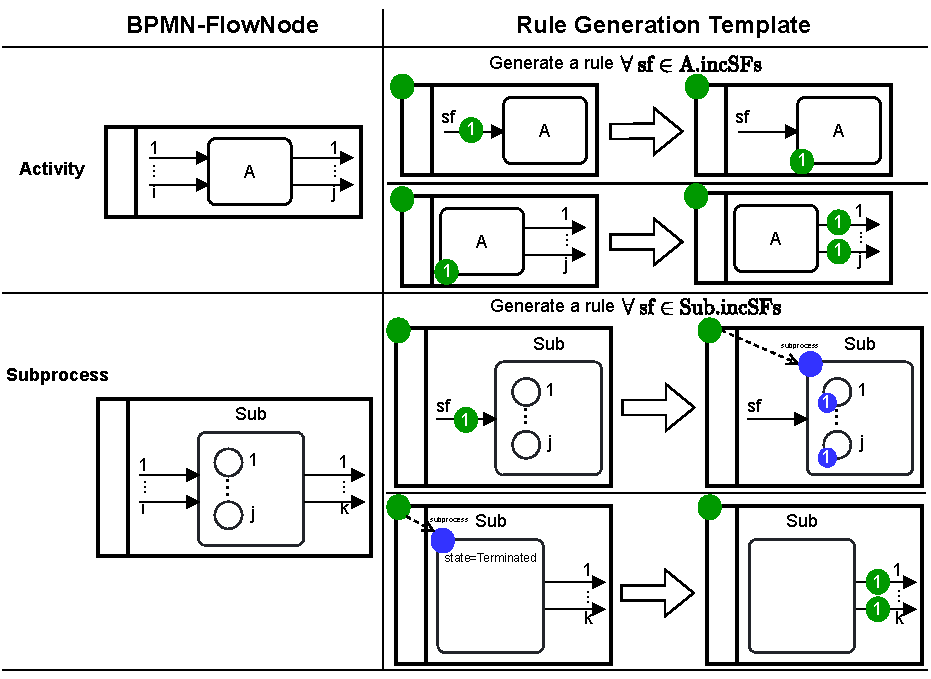
\includegraphics[width=1\textwidth]{images/activities_template.pdf}
    \caption{Rule generation template for activities and subprocesses}
    \label{fig:activityTemplates}
\end{figure}

% Subprocesses/Call activities
Subprocess execution is similar to activity execution.
The upper template generates one rule for each incoming sequence flow.
The rule deletes an incoming token and adds a process snapshot representing a subprocess. 
The addition of this process snapshot is represented with a colored circle on the top left corner of the subprocess with a token at each of its start events.
We added a \textit{subprocess} link between the process snapshots to depict the \textsf{subprocesses} relation in \autoref{fig:typeGraph}.
If the subprocess has no start events, a token for every activity and gateway without incoming sequence flows is added. %, as defined in the BPMN specification.

The bottom rule template generates one rule to delete a terminated process snapshot and adds tokens at each outgoing sequence flow.
Subprocesses are terminated by a generic rule (see section \ref{subsec:instAndTermination}) if they neither have tokens nor subprocesses.


% Send/Receive tasks (mentioned/shown with message events later)
\subsection{Gateways}
\autoref{fig:gatewayTemplates} depicts the rule generation templates for parallel and exclusive gateways (see \autoref{fig:bpmnfeaturesOverview}).
% Parallel
A parallel gateway can synchronize and fork the control flow simultaneously.
Thus, one rule is generated that deletes one token from each incoming sequence flow and adds one token to each outgoing sequence flow.

\begin{figure}[ht]
    \centering
    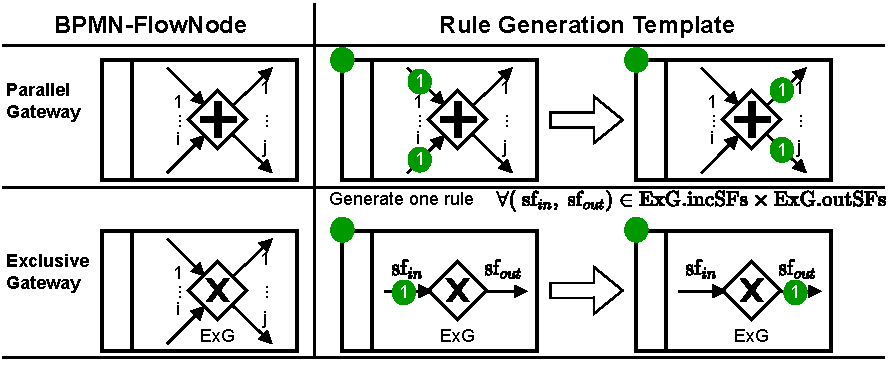
\includegraphics[width=1\textwidth]{images/gateways_template.pdf}
    \caption{Rule generation template for gateways}
    \label{fig:gatewayTemplates}
\end{figure}

% Exclusive --> Exception no incoming flows in sub-processes (token taken from gateway directly)
Exclusive Gateways are triggered by exactly one incoming sequence flow, and exactly one outgoing sequence flow is triggered.
Thus, one rule must be generated for every combination of incoming and outgoing sequence flows.
However, the resulting rule is simple since it only deletes a token from an incoming sequence flow and adds a token to an outgoing sequence flow.

% Event-based with different event combinations
% Mention unsupported types?
\subsection{Message Events}
% Message throw
\autoref{fig:throwEventTemplates} depicts the rule generation templates for \textit{message intermediate throw events} (\textsf{MITE} in \autoref{fig:bpmnfeaturesOverview}).
% Message throw with intermediate catch message events
The upper rule describes how MITEs interact with \textit{message intermediate catch events} (\textsf{MICE} in \autoref{fig:bpmnfeaturesOverview}).
A MITE deletes an incoming token and adds a token at each outgoing sequence flow.
In addition, it sends one message to each waiting process by adding it to the incoming messages of the process.
However, sending each message is optional, meaning that if a process is not ready to consume a message immediately, the message is not added.
%This behavior corresponds to the BPMN semantics \cite{objectmanagementgroupBusinessProcessModel2013}.
We implement optional message sending using a nested rule with quantification.
Concretely, we use an optional existential quantifier (see blue dotted rectangle marked with optional in \autoref{fig:throwEventTemplates}) to send a message only if the receiving process runs and is ready to receive it \cite{rensinkNestedQuantificationGraph2006}.

\begin{figure}[ht]
    \centering
    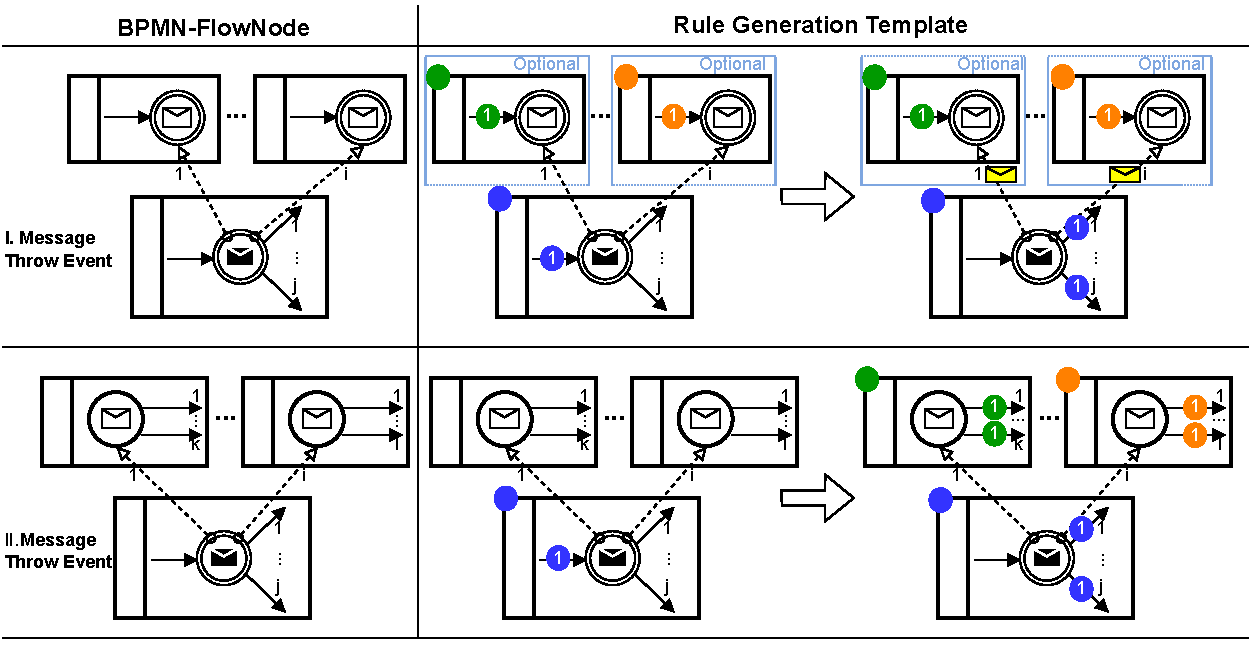
\includegraphics[width=1\textwidth]{images/throw_messages.pdf}
    \caption{Rule generation template for message throw events}
    \label{fig:throwEventTemplates}
\end{figure}

% Message throw with message start events
The bottom rule shows how MITEs trigger new process instances when interacting with \textit{message start events}.
For each receiving \textit{message start event}, a new process snapshot with one token at each outgoing sequence flow is added.
We chose to create a process snapshot immediately rather than creating a message and then consume this message and create a process snapshot in a separate rule.
This decision keeps the rule generation simpler and the state space of the \gls*{gt} system smaller.
It is worth noting that a MITE might interact with MICEs and \textit{message start events} \textit{simultaneously}.
Thus, the rule generation templates in \autoref{fig:throwEventTemplates} can be mixed, i.e., messages can be sent and processes instantiated by one MITE.
We only separated message throw behavior into two rule templates for presentation purposes.
This template generates the MITE rule in \autoref{fig:messageEventRules}.
% Explain the similarity to Send-tasks.
Furthermore, \textit{message end events} and \textit{send tasks} behave similarly regarding message creation and process instantiation.

% Message catch + Receive Task
\autoref{fig:catchMessageTemplates} depicts the rule generation templates for MICEs and \textit{receive tasks}.
To trigger a MICE or a \textit{receive task}, only one message at an incoming \textit{message flow} is needed.
Thus, one rule is generated for each incoming \textit{message flow}.
The upper rule template shows that MICEs delete one message and one token, and add a token at each outgoing sequence flow.
This template generates the MICE rule in \autoref{fig:messageEventRules}.
In the bottom rule template, one can see that \textit{receive task} rules are identical to the \textit{activity} rules in \autoref{fig:activityTemplates},  besides message deletion when a \textit{receive task} starts.

\begin{figure}[ht]
    \centering
    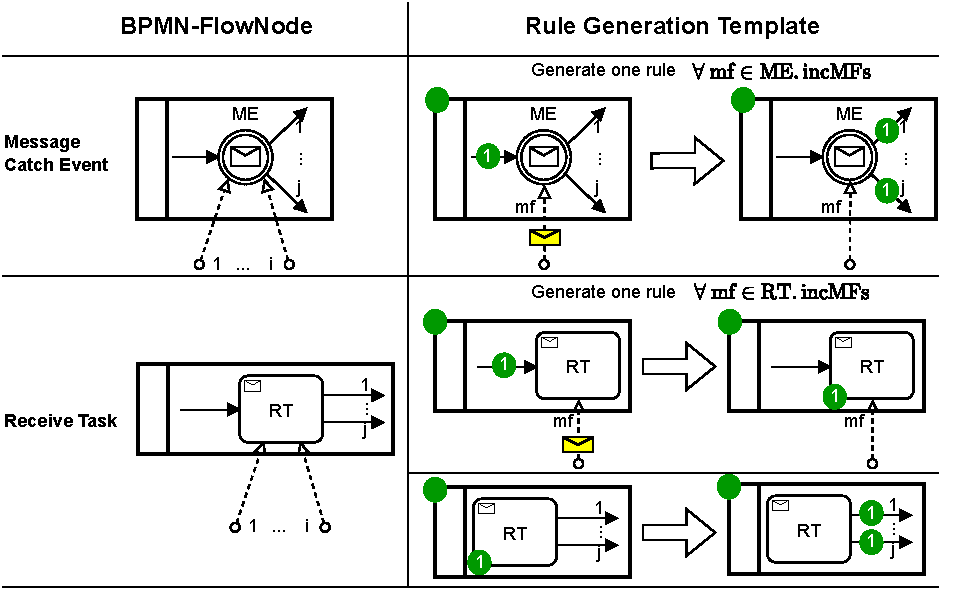
\includegraphics[width=1\textwidth]{images/catch_messages.pdf}
    \caption{Rule generation template for message catch events and receive tasks}
    \label{fig:catchMessageTemplates}
\end{figure}


\section{Model checking BPMN} \label{sec:modelChecking}

Model checking a BPMN model is possible using the generated \gls*{gt} system.
Besides a \gls*{gt} system, a set of temporal properties to be checked and the atomic propositions used in these properties must be supplied.
An atomic proposition is formalized as a graph and holds in a given state if a match exists from the underlying graph of the proposition to the graph representing the state.
This enables model checking of temporal properties using the defined atomic propositions.

We differentiate between \emph{BPMN-specific properties} defined for all BPMN models and \emph{custom properties} tailored towards a particular BPMN model.
We do not consider structural properties (like conformance to the syntax of PBMN) since they can be checked using a standard modeling tool without implementing execution semantics.
We will now give an example of two predefined BPMN-specific properties and show how they can be checked using our approach.
Then, we describe how custom properties can be featureed and checked.

\subsection{BPMN-specific properties}
\textit{Safeness} and \textit{Soundness} properties are defined for BPMN in \cite{corradiniClassificationBPMNCollaborations2018}.
A BPMN model is \emph{safe} if, during its execution, at most one token occurs along the same sequence flow \cite{corradiniClassificationBPMNCollaborations2018}.
Soundness is further decomposed into (i) \emph{Option to complete}: any running process instance must eventually complete, (ii) \emph{Proper completion}: at the moment of completion, each token of the process instance must be in a different end event, as well as (iii) \emph{No dead activities}: any activity can be executed in at least one process instance \cite{corradiniClassificationBPMNCollaborations2018}.
For example, we will describe how to implement the \emph{Safeness} and \emph{Option to complete} properties.

% Safeness
\textbf{Safeness} is specified using the CTL property defined in \eqref{eq:safeness}.
The atomic property \textsf{Unsafe} is true if two tokens of one process snapshot point to the same sequence flow.
Groove rules for all the atomic propositions are included in \cite{krauterArtifactsICGT2023}.

% Option to complete
\emph{Option to complete} is specified using the CTL property defined in \eqref{eq:optionToComplete}.
The atomic proposition \textsf{AllTerminated} is true if there exists no process snapshot in the state \textsf{Running}, i.e., all process snapshots are \textsf{Terminated}.

\noindent\begin{minipage}{.5\linewidth}
\begin{equation} \label{eq:safeness}
  AG(\neg \,\text{Unsafe})
\end{equation}
\end{minipage}%
\begin{minipage}{.5\linewidth}
\begin{equation} \label{eq:optionToComplete}
  AF(\text{AllTerminated}) 
\end{equation}
\end{minipage}
\vskip.3\baselineskip

Checking the properties \textit{Safeness}, \textit{Option to Complete} and \textit{No Dead Activities} is implemented in our tool \cite{krauterArtifactsICGT2023}.
The property \textit{Proper Completion} is not yet implemented but all the information needed can be found in the \gls*{gt} systems state space.

\subsection{Custom properties} \label{subsec:customProperties}
% Defining atomic propositions in BPMN is a novelty.
To make model checking user-friendly, we envision users defining atomic propositions in the extended BPMN syntax, i.e., the concrete syntax introduced in \autoref{fig:typeGraph}.
Thus, to define an atomic proposition, a user adds process snapshots and tokens for a BPMN model, which we can automatically convert to a graph representing an atomic proposition.

For example, the token distribution shown in \autoref{fig:atomicProposition} defines two running process snapshots with a token in task A.
Differently colored tokens define different process snapshots.
A user could use this property, for example, to check if, eventually, two processes are executing task A simultaneously.
Thus, a user does not need to be aware of the \gls*{gt} semantics used for execution, which is a significant advantage compared to other approaches.

\begin{figure}[ht]
    \centering
    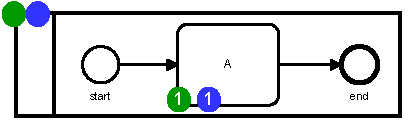
\includegraphics[width=0.45\textwidth]{images/bpmn_semantics-atomic-proposition.pdf}
    \caption{Token distribution defining an atomic proposition.}
    \label{fig:atomicProposition}
\end{figure}


\section{Implementation} \label{sec:impl}

% Tool
Our approach is implemented in a web-based tool.
The tool is open-source, publicly available, and does not require any installation \cite{krauterArtifactsICGT2023}\footnote{\url{https://github.com/timKraeuter/ICGT-2023}}.
\autoref{fig:implScreenshot} depicts a screenshot of the implemented tool.

First, one has to model or upload a \gls*{bpmn} process.
Then, in the verification section one can choose to check either \gls*{bpmn}-specific properties or custom CTL properties.
Finally, our tool can generate a \gls*{gt} system for the supplied \gls*{bpmn} model and run model checking in Groove.
% Evaluation
Furthermore, to evaluate the correctness of our \gls*{hot}, we created a comprehensive test suite, which verifies correct rule generation for the implemented \gls*{bpmn} features \cite{krauterArtifactsICGT2023}.

% Potentially move to the appendix.
\begin{figure}[ht]
    \centering
    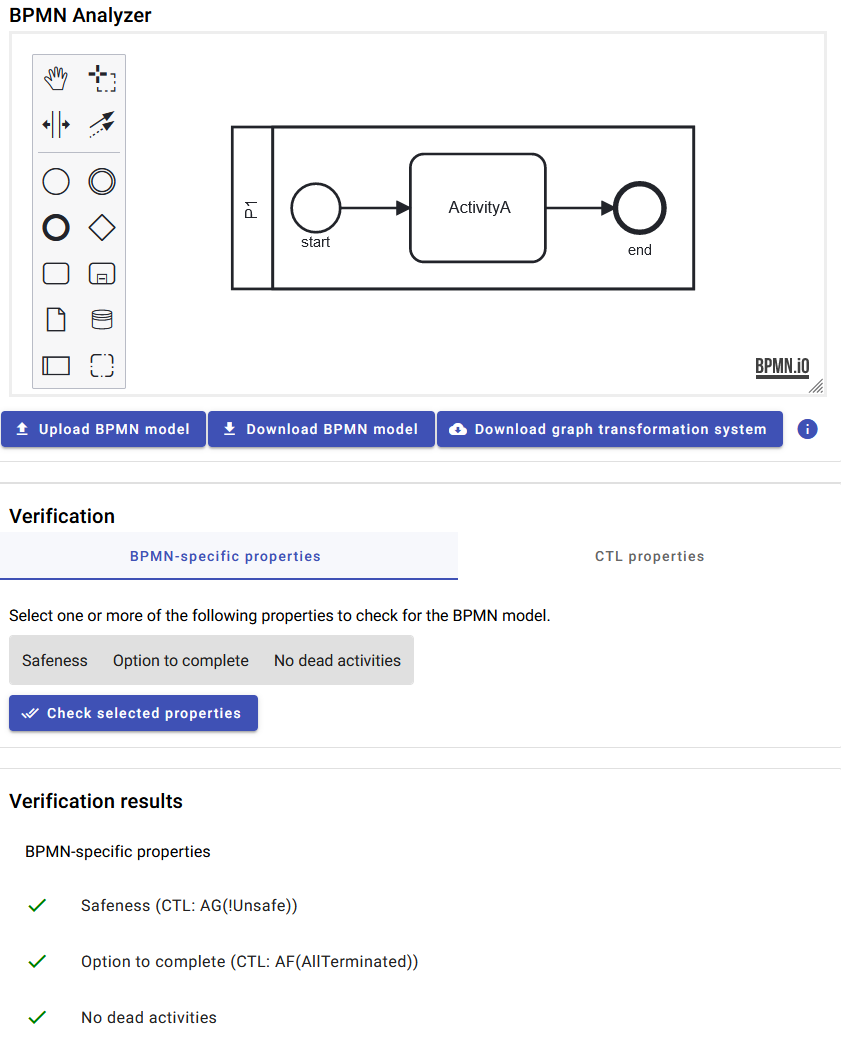
\includegraphics[width=0.8\textwidth]{images/impl.png}
    \caption{Screenshot of the tool}
    \label{fig:implScreenshot}
\end{figure}

\section{Related work} \label{sec:relatedWork}
% Van gorp
A BPMN formalization based on in-place \gls*{gt} rules is given in \cite{vangorpVisualTokenbasedFormalization2013}.
The formalization covers a substantial part of the BPMN specification, including complex concepts such as inclusive gateway merge and compensation.
In addition, the \gls*{gt} rules are visual and thus can easily be aligned with the informal description of the execution semantics of BPMN.
A key difference to our approach is that the rules in \cite{vangorpVisualTokenbasedFormalization2013} are general and can be applied to any BPMN model, while we generate specific rules for every BPMN model using our \gls*{hot}.
Thus, our approach can be seen as a program specialization compared to \cite{vangorpVisualTokenbasedFormalization2013} since we process a concrete BPMN model before its execution.
The \gls*{gt} rules are implemented in a prototype using GrGen.NET.
Moreover, they do \textit{not} support model checking since their goal is only formalization.

% BProve/Corradini
The tool \textit{BProVe} is based on formal BPMN semantics given in rewriting logic and implemented in the Maude system \cite{corradiniFormalApproachAnalysis2021}.
Using this formal semantics, they can verify custom LTL properties and BPMN-specific properties, such as Safeness and Soundness.

% fbpmn/Houhou
The verification framework \textsf{fbpmn} uses first-order logic to formalize and check BPMN models \cite{houhouFirstOrderLogicSemantics2019,houhouFirstOrderLogicVerification2022}.
This formalization is then realized in the TLA\textsuperscript{+} formal language and can be model-checked using TLC.
Like BProVe, \textsf{fbpmn} allows checking BPMN-specific properties, such as Safeness and Soundness.
Furthermore, they focus on different communication models besides the standard in the \gls*{bpmn} specification and support time-related constructs.
We currently disregard data flow (see \cite{corradiniFormalisingAnimatingMultiple2022,el-saberCMMICMComplianceChecking2015}) and time-related constructs (see \cite{duranVerifyingTimedBPMN2017,houhouFirstOrderLogicVerification2022}).

\autoref{tab:supportedfeatures} shows which BPMN features are supported by the approaches mentioned above compared to ours.
We investigated these three approaches since they support a significant subset of the BPMN features and have accessible and well-documented tools.
The coverage of BPMN features greatly impacts how useful each approach is in practice.

\begin{table}[htbp]
    \caption{features supported by different BPMN formalizations (overview based on \cite{vangorpVisualTokenbasedFormalization2013}).}
    \label{tab:supportedfeatures}
    \begin{threeparttable}
    \begin{tabular}{l l l l l}
    \hline
      Feature & Van Gorp &  Corradini & Houhou & This\\
      & et al. \cite{vangorpVisualTokenbasedFormalization2013} & et al. \cite{corradiniFormalApproachAnalysis2021}& et al. \cite{houhouFirstOrderLogicVerification2022} & paper\\
      \hline
      \textit{Instantiation and termination} & &\\
      Start event instantiation & X & X & X & X\\
      Exclusive event-based gateway instantiation & X & & & X\\
      Parallel event-based gateway instantiation &  & & & \\
      Receive task instantiation & & & & X\\
      Normal process completion & X & X & X & X\\
      \textit{Activities} & & & &\\
      Activity & X & X & X & X\\
      Subprocess & X & & X & X\\
      Ad-hoc subprocesses & & & &\\
      Loop activity & X & & &\\
      Multiple instance activity & & & & \\
      \textit{Gateways} & & & &\\
      Parallel gateway & X & X & X & X\\
      Exclusive gateway & X & X & X & X\\
      Inclusive gateway (split) & X & X & X & X\\
      Inclusive gateway (merge) & X & & X & X\\
      Event-based gateway &  & X\tnote{1} & X & X\\ % No timer and conditional events after event based gateway supported.
      Complex gateway & & & &\\
      \textit{Events} & & & & \\
      None Events & X & X & X & X\\
      Message events & X & X & X & X\\
      Timer Events & & & X & \\
      Escalation Events & & & & X\\
      Error Events & X & & & X\\
      Cancel Events & X & & &\\
      Compensation Events & X & & &\\
      Conditional Events & & & &\\
      Link Events & X & & & X\\
      Signal Events & X & & & X\\
      Multiple Events &  & & & \\
      Terminate Events & X & X & X & X\\
     Boundary Events & X\tnote{2} & & X\tnote{3} & X\\ % To the same extent as the event support
      Event subprocess &  &  &  & X\\
    \end{tabular}
    \begin{tablenotes}
        \item[1] Does not support receive tasks after event-based gateways.
        \item[2] Only supports interrupting boundary events on tasks, not subprocesses.
        \item[3] Only supports message and timer events.
    \end{tablenotes}
    \end{threeparttable}
\end{table}

% Summarize the findings and explain them in more detail
Our approach covers most of the \gls*{bpmn} features compared to other current approaches.
Thus, we conclude that our formalization is comprehensive but can still be improved.
In addition, it covers the most important features found in practice since we come close to the feature coverage of popular process engines such as Camunda\footnote{\url{https://docs.camunda.org/manual/7.16/reference/bpmn20/}}.

\section{Conclusion \& future work} \label{sec:conclusion}
This paper makes two main practical contributions.
First, we conceptualized a new approach utilizing a \gls*{hot} to formalize the semantics of behavioral languages.
Our approach moves complexity from the \gls*{gt} rules to the rule templates making up the \gls*{hot}.
Furthermore, the approach can be applied to any behavioral language if one can define its state structure and identify its state-changing elements.

Second, we apply our approach to BPMN, resulting in a comprehensive formalization regarding feature coverage (compared to the literature and industrial process engines) that supports checking behavioral properties.
Furthermore, our contribution resulted in an open-source web-based tool to make our ideas easily accessible to other researchers and potential practitioners.

Potential future work can target both of our main contributions.
First, we plan a detailed comparison of our \gls*{hot} approach with an approach with fixed rules.
It will be interesting to investigate how the two approaches differ, for example, in runtime during state space generation.
Second, we aim to improve our formalization and the resulting tool in multiple ways.
We intend to extend our formalization to support the remaining few BPMN features used in practice.
For example, we want to support cancel and compensation events.
Furthermore, we intend to extend the features of our tool so that the user can define atomic propositions for model checking directly in the tool, as described in \autoref{sec:modelChecking}.
Finally, we want to turn the modeling environment of our tool into an interactive simulation environment that is driven by our formal semantics.
In addition, we can use this environment to visualize potential counterexamples of behavioral properties.

\bibliographystyle{splncs04} 
\bibliography{bib}
\end{document}
